Trình điều khiển thiết bị (Driver) là thành phần phần mềm chính của thiết bị. Hoạt động của mô đun này được mô tả trong hình \ref{driver-block}. Luồng điều khiển liên tục chạy và thay đổi trạng thái màn hình tùy theo dữ liệu người dùng nhập như khi người dùng thay đổi nội dung, thay đổi trạng thái màn hình hay khi thực hiện cuộn văn bản.

Dữ liệu driver được cập nhật bởi người dùng thông qua hệ thống sysfs. Dữ liệu trạng thái sau khi cập nhật sẽ được cập nhật bởi luồng điều khiển và hiển thị trên màn hình LCD1602.

\begin{figure}[H]
	\centering
	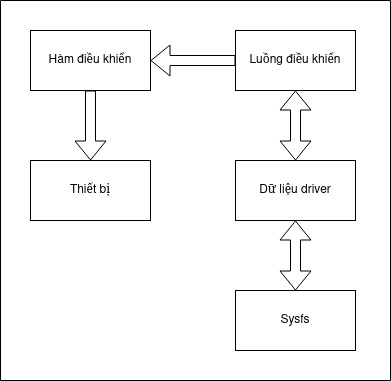
\includegraphics[width=0.8\textwidth]{../images/driver.jpg}
	\caption{Sơ đồ khối của trình điều khiển thiết bị}
	\label{driver-block}
\end{figure}

Luồng điều khiển chính được mô tả trong hình \ref{main-thread}. Do luồng trong không gian nhân không thể kết thúc một cách tự động hoặc kết thúc từ luồng khác mà chỉ có thể gửi tín hiệu kết thúc đến nó nên các câu lệnh phải được đặt bên trong vòng lặp kiểm tra trạng thái kết thúc. Bên trong vòng lặp, thực hiện lấy dữ liệu hiển thị và gọi hàm hiển thị tương ứng nếu dữ liệu có sự thay đổi. Sau đó gọi hàm làm mới dữ liệu và tạm dừng luồng trong 1 giây để chuyển sang vòng lặp tiếp theo.

\begin{figure}[H]
	\centering
	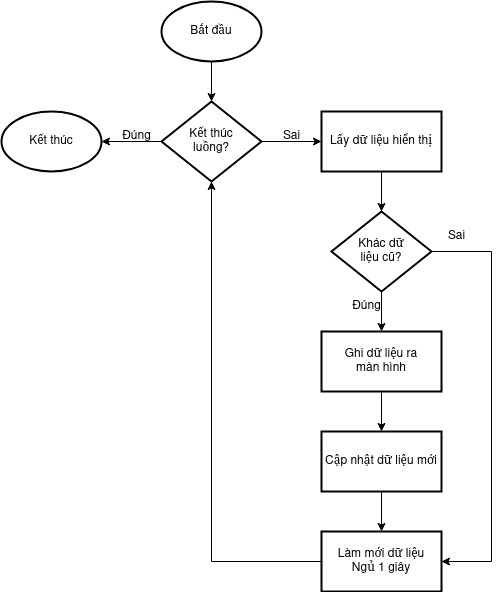
\includegraphics[width=0.8\textwidth]{../images/driver-work-thread.jpg}
	\caption{Hoạt động của luồng điều khiển chính}
	\label{main-thread}
\end{figure}

Người dùng thực hiện thao tác với màn hình qua hệ thống file ảo của sysfs bằng việc đọc hoặc ghi vào chúng. Thao tác này có thể thực hiện trực tiếp trên shell nên có thể lập trình giao tiếp qua các dịch vụ từ xa như Secure Shell. Các file nằm trong đường dẫn /sys/kernel/pcf\_lcd.
\begin{table}[H]
	\centering
	\caption{Danh sách file sysfs}
	\begin{tabular}{|c|c|}
		\hline
		\textbf{Tên file} & \textbf{Chức năng}\\
		\hline
		content & đọc hoặc ghi nội dung hiển thị\\
		line1 & đọc nội dung dòng 1\\
		line2 & đọc nội dung dòng 2\\
		scroll & bật/tắt chế độ cuộn văn bản\\
		auto\_newline & bật/tắt chế độ tự động xuống dòng\\
		backlight & bật/tắt đèn nền \\
		cursor & bật/tắt con trỏ \\
		blink & bật/tắt nháy con trỏ\\
		display & bật/tắt hiển thị\\
		\hline		
	\end{tabular}
\end{table}